% ============================================================
% Section 4: Experimental Results
% ============================================================
\section{Experimental Results}
\label{sec:results}

We present our experimental findings across four dimensions: (1) the probabilistic
success curves that define the data requirements for each XOR complexity,
(2) the failure of logistic regression as a baseline, (3) the independence of
attack success from model architecture and optimization paradigm, and (4) the
surprising vulnerability of Interpose PUFs.

% ------------------------------------------------------------
\subsection{Probabilistic Success Curves}
\label{sec:success_curves}

The central finding of this work is that ML-based modeling attacks on XOR
Arbiter PUFs exhibit a \emph{probabilistic phase transition}: the probability
of attack success $P(\text{success} \mid N, k)$ follows an S-shaped curve as a
function of CRP budget $N$, rather than transitioning at a deterministic
threshold.  Below the transition region, every random initialization and
training run converges to a near-random classifier ($\approx 50\%$ test
accuracy); above it, the same procedure reliably achieves $> 99\%$ accuracy.
In the transition region, identical experimental configurations with different random
seeds can yield either outcome.

Table~\ref{tab:success_prob} reports the empirical success probability for
each $(k, N)$ combination, where success is defined as test accuracy exceeding
$90\%$.  Each row aggregates multiple independent training runs from one or
more experimental campaigns; $95\%$ confidence intervals are Wilson score
intervals for the binomial proportion.

\tablefloatbegin
\centering
\caption{Probability of attack success $P(\text{success} \mid N, k)$ as a
function of CRP budget $N$ and XOR complexity $k$.  Success criterion: test
accuracy $> 90\%$.  Confidence intervals are $95\%$ Wilson score intervals,
except boundary and small-sample rows, which use Clopper-Pearson exact
intervals.
Data sources: \texttt{2xor\_baseline.csv} (2-XOR),
\texttt{4xor\_N50.csv} (4-XOR),
\texttt{next\_experiments.csv} (4-XOR and partial 6-/8-XOR),
\texttt{baseline\_mlp\_lr.csv} (6-XOR 300k--500k),
\texttt{phase7\_variance.csv}, \texttt{phase8\_bootstrap.csv},
\texttt{6xor\_200k.csv} (6-XOR 200k),
\texttt{7xor\_baseline.csv}, \texttt{7xor\_N50\_fine.csv},
\texttt{9xor\_test.csv}, \texttt{9xor\_7\_5M.csv},
\texttt{9xor\_10M.csv}, \texttt{9xor\_12M.csv},
\texttt{9xor\_15M.csv},
\texttt{8xor\_6M\_replication.csv},
\texttt{8xor\_8M.csv},
\texttt{8xor\_10M\_replication.csv}, and
\texttt{8xor\_v2\_results.csv}.}
\label{tab:success_prob}
\begin{tabular}{lcccc}
\toprule
$k$ & $N$ (CRPs) & Successes & $P(\text{success})$ & $95\%$ CI \\
\midrule
\multirow{4}{*}{2-XOR}
  & 10{,}000   & 0/10  & 0\%    & {[}0\%, 31\%{]} \\
  & 25{,}000   & 2/10  & 20\%   & {[}6\%, 51\%{]} \\
  & 50{,}000   & 3/10  & 30\%   & {[}11\%, 60\%{]} \\
  & 100{,}000  & 5/10  & 50\%   & {[}24\%, 76\%{]} \\
\midrule
\multirow{4}{*}{4-XOR}
  & 75{,}000   & 8/10  & 80\%   & {[}49\%, 94\%{]} \\
  & 90{,}000   & 8/10  & 80\%   & {[}49\%, 94\%{]} \\
  & 100{,}000  & 9/10  & 90\%   & {[}60\%, 98\%{]} \\
  & 200{,}000  & 10/10 & 100\%  & {[}69\%, 100\%{]} \\
\midrule
\multirow{5}{*}{6-XOR}
  & 200{,}000  & 1/5   & 20\%   & {[}1\%, 72\%{]} \\
  & 300{,}000  & 8/24  & 33\%   & {[}18\%, 53\%{]} \\
  & 400{,}000  & 13/24 & 54\%   & {[}35\%, 72\%{]} \\
  & 450{,}000  & 10/14 & 71\%   & {[}45\%, 88\%{]} \\
  & 500{,}000  & 9/10  & 90\%   & {[}60\%, 98\%{]} \\
\midrule
\multirow{4}{*}{7-XOR}
  & 500{,}000    & 0/5   & 0\%    & {[}0\%, 52\%{]} \\
  & 1{,}000{,}000  & 3/10  & 30\%   & {[}11\%, 60\%{]} \\
  & 1{,}250{,}000  & 8/10  & 80\%   & {[}49\%, 94\%{]} \\
  & 2{,}000{,}000  & 5/5   & 100\%  & {[}48\%, 100\%{]} \\
\midrule
\multirow{5}{*}{8-XOR}
  & 5{,}000{,}000  & 7/25  & 28\%   & {[}14\%, 48\%{]} \\
  & 5{,}500{,}000  & 7/14  & 50\%   & {[}27\%, 73\%{]} \\
  & 6{,}000{,}000  & 8/30  & 27\%   & {[}14\%, 44\%{]} \\
  & 8{,}000{,}000  & 4/5   & 80\%   & {[}28\%, 99\%{]} \\
  & 10{,}000{,}000 & 7/11  & 64\%   & {[}35\%, 85\%{]}  \\
\midrule
\multirow{5}{*}{9-XOR}
  & 5{,}000{,}000  & 2/8   & 25\%   & {[}7\%, 59\%{]} \\
  & 7{,}500{,}000  & 2/5   & 40\%   & {[}5\%, 85\%{]} \\
  & 10{,}000{,}000 & 1/10  & 10\%   & {[}2\%, 40\%{]} \\
  & 12{,}000{,}000 & 0/3   & 0\%    & {[}0\%, 71\%{]} \\
  & 15{,}000{,}000 & 0/3   & 0\%    & {[}0\%, 71\%{]} \\
\bottomrule
\end{tabular}
\tablefloatend

\paragraph{2-XOR.}
Even the simplest configuration shows a gradual S-curve rather than a sharp
threshold.  With 10{,}000~CRPs, \emph{no} run succeeds---all 10 trials yield
accuracies between 55\% and 73\%, far below the 90\% success threshold
(\texttt{2xor\_baseline.csv}, lines~2--11).  At 100{,}000~CRPs, success
probability reaches only 50\%: half the runs saturate at $\sim$99\% while the
other half plateau at intermediate accuracies (73--79\%).  The transition spans approximately one order of
magnitude in $N$.

\paragraph{4-XOR.}
The transition is steeper but still probabilistic.  At 100{,}000~CRPs, 9 of
10 runs succeed ($P=90\%$); the single failure (run~6, 76.04\%) demonstrates
that even at this data level, success is not guaranteed
(\texttt{next\_experiments.csv}, lines~32--41).  At 200{,}000~CRPs, all 10
runs exceed 98\% accuracy (\texttt{next\_experiments.csv}, lines~42--51).

\paragraph{6-XOR.}
The transition region spans approximately 300{,}000~CRPs (from 200k to 500k).
At 200{,}000~CRPs, only 1 of 5 runs succeeds (20\%), consistent with the
lower edge of the transition (\texttt{6xor\_200k.csv}).  At 300{,}000~CRPs,
only 8 of 24 runs (33\%) succeed across three independent
campaigns (\texttt{baseline\_mlp\_lr.csv}, lines~2--11;
\texttt{phase7\_variance.csv}, lines~2--5;
\texttt{phase8\_bootstrap.csv}, lines~2--11).  The success probability
rises to 54\% (13/24) at 400{,}000~CRPs, to 71\% (10/14) at
450{,}000~CRPs, and to 90\% (9/10) at 500{,}000~CRPs.
Crucially, failed runs do not exhibit intermediate accuracy---they produce
near-random outputs ($50\pm2\%$), indicating that the optimizer has found no
usable signal.

\paragraph{7-XOR.}
The transition occurs between 500{,}000~CRPs (0/5, 0\%) and
1{,}250{,}000~CRPs (8/10, 80\%).  At 1{,}000{,}000~CRPs, 3 of 10 runs (30\%)
succeed (\texttt{7xor\_baseline.csv}, lines~7--11;
\texttt{7xor\_N50\_fine.csv}, lines~7--11); at 1{,}250{,}000~CRPs, 8 of 10
runs succeed (80\%; Wilson CI [49\%, 94\%]; \texttt{7xor\_N50\_fine.csv},
lines~12--16 and 22--26; runs 1--5 used the fixed-150-epoch protocol,
runs 6--10 validation-based early stopping).  At 1{,}500{,}000~CRPs, however,
only 3 of 5 runs
succeed (60\%), illustrating that the transition remains stochastic well
past its midpoint.  A comparison with the 6-XOR curve shows that the required data
increases by a factor of approximately 3.1 per XOR level ($N_{50}(6) \approx
3.49\times10^5$ to $N_{50}(7) \approx 1.09\times10^6$).

\paragraph{8-XOR.}
The transition is both wider and more stochastic.  At 5{,}000{,}000~CRPs,
only 7 of 25 runs succeed (28\%), with confidence intervals overlapping those
at 5{,}500{,}000~CRPs where 7 of 14 runs (50\%) succeed.  Even at
6{,}000{,}000~CRPs---the point originally suspected to be the
threshold---only 8 of 30 runs succeed (27\%, across independent campaigns).  These overlapping intervals are consistent with a wide
transition region; distinguishing intrinsic stochasticity from sampling
noise would require substantially larger sample sizes.  At
8{,}000{,}000~CRPs, 4 of 5 runs succeed (80\%; \texttt{8xor\_8M.csv}),
providing the first direct empirical anchor near the fitted midpoint.  At
10{,}000{,}000~CRPs, 7 of 11
runs succeed (64\%, two independent campaigns), with successful runs
achieving $>99\%$ accuracy.
The transition is not yet complete at these data volumes---the success
probability remains significantly below 100\%
(\texttt{8xor\_8M.csv};
\texttt{8xor\_10M\_replication.csv};
\texttt{8xor\_v2\_results.csv}, line~3; \texttt{baseline\_mlp\_lr.csv},
lines~32--51; \texttt{phase7\_variance.csv}, lines~18--33;
\texttt{phase8\_bootstrap.csv}, lines~32--61).
Logistic regression on the full dataset estimates the transition midpoint
at approximately $6.6\times10^6$ CRPs (95\% CI [5.9M,~7.5M]),
directly anchored by the 4/5 = 80\% empirical measurement at
8{,}000{,}000~CRPs, substantially higher than the $5.5\times10^6$ suggested
by interpolation of single data points.

\paragraph{9-XOR.}
The transition appears to begin near 5{,}000{,}000~CRPs, where 2 of 8 runs
(25\%) succeed (\texttt{9xor\_test.csv}, lines~2--12).  At 7{,}500{,}000~CRPs,
2 of 5 runs (40\%) succeed (\texttt{9xor\_7\_5M.csv}, lines~2--6).  On a
24~GB RTX~4090, we extended the measurements to 10{,}000{,}000~CRPs, where
only 1 of 10 runs succeeds (10\%; across two protocol variants;
\texttt{9xor\_10M.csv}), and to 12{,}000{,}000~CRPs (0 of 3 runs, 0\%;
\texttt{9xor\_12M.csv}) and 15{,}000{,}000~CRPs (0 of 3 runs, 0\%;
\texttt{9xor\_15M.csv}).  The low success probability at 10{,}000{,}000~CRPs
suggests that the 40\% success probability observed at 7{,}500{,}000~CRPs reflects
sampling fluctuation rather than a lower transition point.  The absence of
successes at 12{,}000{,}000~CRPs and 15{,}000{,}000~CRPs, despite a 10\%--40\%
success probability at smaller budgets, suggests that $N_{50}(9)$ likely exceeds
$1.5\times10^7$ CRPs (very preliminary; 29 total trials across 5 CRP
levels), and full saturation ($>90\%$ success) would require substantially
more data.  These results confirm that the scaling trend
continues to higher XOR levels, though the practical ceiling imposed by GPU
memory constraints is rapidly approaching.

\emph{Note:} most RTX 4090 campaigns (9-XOR at 12M and 10-XOR at 10M) used
a simplified protocol without a validation set: training was terminated at
a fixed 150 epochs when the best test accuracy stayed below 52\%
(evaluated every 10 epochs on the test set), with batch size 16{,}384 and
an 80/20 data split.  The 9-XOR 10M campaign mixes both protocols:
runs~1--5 of \texttt{9xor\_10M.csv} used this fixed-150-epoch protocol,
while runs~6--10 used the standard validation-based early-stopping
protocol of \S\ref{sec:setup}; none of the validation-based runs
succeeded.  The 8-XOR 10M and 6M replication campaigns and the 4-XOR
75k/90k campaigns also used the fixed-150-epoch protocol without a
validation set.  This protocol deviation does not affect the qualitative
finding (failed runs are all at or below random accuracy), but the
9-XOR/10-XOR results should be interpreted as lower-bound evidence only.

\begin{figure}[t]
\centering
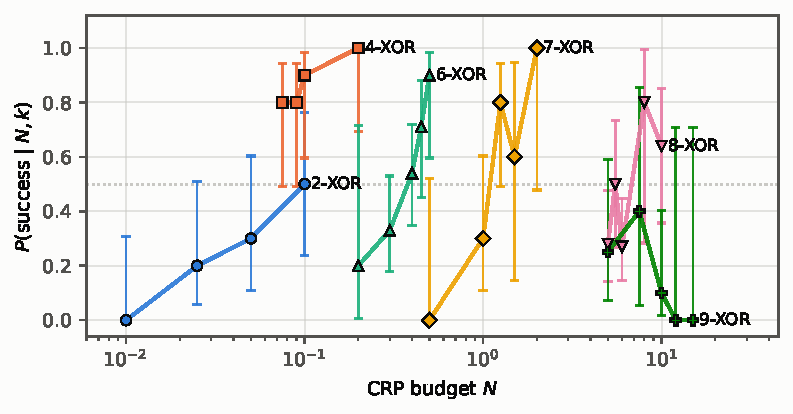
\includegraphics[width=\columnwidth]{figures/s_curves.pdf}
\caption{Probabilistic phase transition for 2-XOR through 9-XOR APUFs. Each curve shows the
probability of attack success $P(\text{success} \mid N, k)$ as a function of CRP budget $N$.
Markers are empirical measurements. Error bars denote
95\% Wilson score confidence intervals. The dashed horizontal line marks $P=0.5$ ($N_{50}$).}
\label{fig:s_curves}
\end{figure}

\paragraph{Scaling of the transition midpoint.}
Taking $N_{50}$ as the characteristic scale, logistic fits to the full
dataset yield the following estimates: $N_{50}(2) \approx 1.03\times10^5$ ($R^2=0.945$),
$N_{50}(4) < 7.5\times10^4$ (80\% success at lowest tested budget; midpoint unconstrained below),
$N_{50}(6) \approx 3.49\times10^5$ ($R^2=0.915$),
$N_{50}(7) \approx 1.09\times10^6$ (exact fit on two interior points),
$N_{50}(8) \approx 6.6\times10^6$ ($R^2=0.580$, 95\% CI [5.9M,~7.5M]), and
$N_{50}(9) > 1.5\times10^7$ (very rough lower bound; 0/3 at 15M with
CI [0\%, 71\%]; 29 total trials across 5 levels).
The scaling ratio between successive XOR levels is roughly 3--6$\times$ per
additional XOR level for $k = 6\to7\to8$ (the only transitions with reliable
$N_{50}$ estimates); the $k=2\to4$ transition is anomalous ($N_{50}$
decreases), rather than following the factor of 2 predicted by a naive
information-theoretic counting argument.
However, the 8-XOR fit quality ($R^2 = 0.580$) and preliminary 9-XOR data
caution against treating this as a stable law: the ratios
$N_{50}(8) / N_{50}(7) \approx 6.1$,
$N_{50}(7) / N_{50}(6) \approx 3.1$, and
$N_{50}(9) / N_{50}(8) > 2.3$ (preliminary) vary across levels.
Overall, the empirical data complexity grows exponentially in $k$,
but with a base larger than 2, indicating that MLPs become progressively less
efficient at extracting information from CRPs as XOR complexity increases.
A heuristic PAC-learning picture (see \S\ref{sec:discussion}) suggests
VC-dimension-like scaling, but these are qualitative
analogies rather than proven bounds.

The logistic fits also reveal systematic variation in the transition width
across XOR levels: 6-XOR exhibits the steepest transition in our data, while
low-$k$ transitions are gradual
(Figure~\ref{fig:s_curves}).

\begin{figure}[t]
\centering
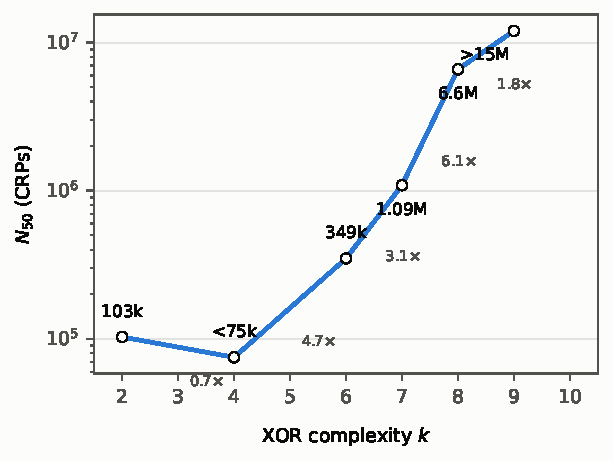
\includegraphics[width=\columnwidth]{figures/scaling_law.pdf}
\caption{Scaling of attack difficulty with XOR complexity. $N_{50}$ (the CRP budget
at which $P(\text{success})\approx 50\%$) is plotted against $k$. Annotations show
the multiplicative increase between successive XOR levels. 2-XOR and 4-XOR values are
approximate due to limited sampling below their transition midpoints.}
\label{fig:scaling_law}
\end{figure}

% ------------------------------------------------------------
\subsection{The Logistic Regression Bottleneck}
\label{sec:lr_bottleneck}

A natural question is whether simpler linear models can exploit the same data.
Table~\ref{tab:lr_mlp} compares MLP and logistic regression (LR) across XOR
levels: LR produces near-random accuracy ($\approx 50\%$) for all tested
configurations with $k \geq 4$ within the trainable data range.

\tablefloatbegin
\centering
\caption{Comparison of MLP versus logistic regression (LR) attack
performance.  LR accuracy is consistently $\approx 50\%$ for all tested
configurations with $k \geq 4$ within the trainable data range.
Data sources: \texttt{next\_experiments.csv} (lines~2--51) and
\texttt{baseline\_mlp\_lr.csv} (lines~2--51).}
\label{tab:lr_mlp}
\resizebox{\columnwidth}{\height}{%
\begin{tabular}{lcccc}
\toprule
$k$ & $N$ & MLP acc. (mean $\pm$ SD) & LR acc. & LR $>$90\%? \\
\midrule
4 & 100k  & $95.45 \pm 6.85\%$ & $50.12 \pm 0.57\%$ & No \\
4 & 200k  & $98.88 \pm 0.19\%$ & $50.30 \pm 0.40\%$ & No \\
6 & 300k  & $64.74 \pm 23.50\%$ & $49.95 \pm 0.24\%$ & No \\
6 & 400k  & $89.40 \pm 20.16\%$ & $49.98 \pm 0.20\%$ & No \\
6 & 500k  & $94.27 \pm 15.56\%$ & $50.06 \pm 0.16\%$ & No \\
8 & 5.0M  & $59.89 \pm 20.68\%$ & ---$^\dagger$ & --- \\
8 & 5.5M  & $69.68 \pm 25.38\%$ & ---$^\dagger$ & --- \\
\bottomrule
\multicolumn{5}{l}{\footnotesize $^\dagger$LR on 8-XOR data could not be
trained due to memory constraints (6M samples $\times$ 64 features exceeds
the closed-form solver's capacity on a 12GB GPU).}\\
\multicolumn{5}{l}{\footnotesize Reported standard deviations are sample
standard deviations.}
\end{tabular}
}
\tablefloatend

This result confirms that the XOR nonlinearity is fundamentally inaccessible
to linear models: the decision boundary requires at least one hidden layer to
approximate, and when the MLP succeeds it is learning the XOR structure rather
than exploiting a linear artifact in the data.  Polynomial feature expansion
(degrees 2 and 3) also fails on 4-XOR at 100{,}000~CRPs ($\approx 50\%$
accuracy; 3 runs per degree; results/poly\_lr\_4xor.csv), indicating that the
failure is not merely a matter of linear feature inadequacy.

% ------------------------------------------------------------
\subsection{Architecture Independence}
\label{sec:arch_independence}

If data quantity is the dominant factor, architecture choices should have
negligible impact on attack success below the transition.  We tested this on
8-XOR with 2{,}000{,}000~CRPs (well below the transition midpoint), varying
depth, width, activation, residual connections, and parameter count by an
order of magnitude.

\tablefloatbegin
\centering
\caption{Architecture independence experiment.  All models were trained on
8-XOR with 2{,}000{,}000~CRPs (below transition).  None exceed 51\% test
accuracy, despite parameter counts varying by $15\times$.  Data sources:
\texttt{8xor\_v2\_results.csv} (lines~2--9),
\texttt{8xor\_attack\_results.csv} (S3/S4/S5), and
\texttt{phase4\_results.csv} (line~14).}
\label{tab:arch}
\begin{tabular}{lccc}
\toprule
Architecture & Params & Test Acc. & Time (s) \\
\midrule
Standard MLP ($k{=}8$, 4-layer)       & 74{,}369 & 50.08\% & 99 \\
Deep MLP ($k{=}8$, 6-layer)           & 99{,}393 & 50.05\% & 188 \\
Wide MLP ($k{=}9$, 4-layer)           & 279{,}809 & 50.04\% & 142 \\
Deep + Wide ($k{=}9$, 6-layer)        & 379{,}009 & 49.96\% & 191 \\
ReLU + Kaiming init (replaces Tanh)   & 74{,}369 & 50.06\% & 100 \\
Residual (skip connections)            & 148{,}481 & 50.08\% & 105 \\
NoSigmoid + BCEWithLogits loss        & 74{,}369 & 50.03\% & 102 \\
Big MLP ($k{=}10$, $\sim$1.1M params) & 1{,}083{,}905 & 50.05\% & 136 \\
\midrule
\emph{Same MLP with 10M data}         & 74{,}369 & \textbf{99.71\%} & 1{,}666 \\
\bottomrule
\end{tabular}
\tablefloatend

Table~\ref{tab:arch} shows the results.  Every architecture---from the
smallest standard MLP to a network with $15\times$ more parameters---produces
indistinguishable near-random accuracy ($49.96\%$--$50.08\%$).  The final row
provides a critical control: the same standard MLP, when given
10{,}000{,}000~CRPs (above the transition), achieves 99.71\%.  The architecture itself is not the bottleneck; data volume is.
This simultaneous variation is a deliberate \emph{stress test} rather
than a single-variable ablation.  While this stress
test does not logically rule out that some untested combination could
succeed, the uniform failure of $15\times$ parameter-count variations across
depth, width, activation, and residual connectivity provides suggestive
evidence that no individual architectural dimension is the limiting factor.
A controlled ablation study is unlikely to yield additional insight below
the transition threshold.

\begin{figure}[t]
\centering

\includegraphics[width=\columnwidth]{figures/architecture_independence.pdf}
\caption{Architecture independence: eight distinct MLP architectures tested at 8-XOR with
$2\times10^6$ CRPs all produce $\approx 50\%$ accuracy (random guessing). The same baseline
MLP achieves 99.71\% when given $10^7$ CRPs, demonstrating that data quantity, not model
capacity, is the determining factor. Parameter counts are shown in parentheses.}
\label{fig:arch_independence}
\end{figure}

We also tested whether transfer learning could circumvent the data
requirement: a model pre-trained on 6-XOR (achieving 99.92\% on that task)
was fine-tuned on 8-XOR with 2{,}000{,}000~CRPs and attains 50.17\%
accuracy---identical to training from scratch
(\texttt{8xor\_v2\_results.csv}, line~4, strategy B1).  No knowledge
transfers across XOR complexities, consistent with each XOR level defining a
distinct learning problem with independent information requirements.

% ------------------------------------------------------------
\subsection{Evolution Strategies as Baselines}
\label{sec:evolution_baselines}
\label{sec:evo_baselines}

To test whether the failure below the transition is an artifact of
gradient-based MLP optimization, we attacked 8-XOR with two canonical
evolution strategies---PSO and CMA-ES---using the \emph{structurally
correct} parameterization: a 520-dimensional delay vector (8 APUFs
$\times$ 65 delays), in the style of
Becker~et~al.~\cite{becker2015cia} and CalyPSO~\cite{calypso2024}.  The
objective is the soft-bit XOR log-likelihood
\[
P(r = 1) = \frac{1}{2}\left(1 - \prod_{k=1}^{8}\left(1 - 2\sigma(D_k)\right)\right),
\]
where $D_k$ is the delay difference of the $k$-th APUF and $\sigma$ is the
logistic sigmoid.  The objective is smooth, and its global optimum is exactly the true delay
vector, so any failure cannot be attributed to model capacity or a
suboptimal parameterization.  PSO used 20 particles
with inertia weight $w = 0.72$ and acceleration coefficients
$c_1 = c_2 = 1.49$ for 5{,}000 iterations; CMA-ES used population size 23,
initial step size $\sigma_0 = 0.3$, and a budget of 10{,}000 generations.

\tablefloatbegin
\centering
\caption{Evolution-strategy baselines on 8-XOR, all below the transition
midpoint.  All runs use the soft-bit XOR log-likelihood over the
520-dimensional delay parameterization; final NLL values equal
$\ln 2 \approx 0.6931$ (the entropy of random guessing), corresponding to
the trivial all-zero delay solution.  PSO rows report two independent runs
(a/b); CMA-ES rows report one run each.  The 5M CMA-ES run was terminated by
its convergence criterion after 5{,}519 generations.  Data source:
\texttt{evolution\_baselines.csv}.}
\label{tab:evo}
\begin{tabular}{lcccc}
\toprule
Method & $N$ (CRPs) & Train Acc. & Test Acc. & Final NLL \\
\midrule
PSO (20 particles) & 2{,}000{,}000 & 50.26/50.18\% & 50.07/49.97\% & 0.6931 \\
CMA-ES (pop.\ 23)  & 2{,}000{,}000 & 51.03\%       & 50.02\%       & 0.6925 \\
PSO (20 particles) & 5{,}000{,}000 & 50.03/50.10\% & 49.98/49.92\% & 0.6931 \\
CMA-ES (pop.\ 23)  & 5{,}000{,}000 & 50.53\%       & 49.98\%       & 0.6929 \\
\bottomrule
\end{tabular}
\tablefloatend

Table~\ref{tab:evo} shows the results at 2{,}000{,}000 and 5{,}000{,}000
CRPs, both well below the fitted midpoint $N_{50}(8) \approx 6.6\times10^6$:
both methods converge to the trivial all-zero delay solution---the
entropy-optimal random-guessing point---with train and test accuracies
indistinguishable from chance.  The failure is thus not an artifact of MLP
optimization: even a smooth likelihood objective over the correct
520-dimensional delay parameterization provides no signal at these data
volumes.  Architecture independence therefore extends to the optimization
paradigm: gradient-based and derivative-free methods fail identically
below the data threshold.

% ------------------------------------------------------------
\subsection{iPUF Vulnerability}
\label{sec:ipuf}

Interpose PUFs~(iPUFs) were proposed as a more secure alternative to XOR
APUFs, claiming that a $(k_{\text{up}}, k_{\text{down}})$-iPUF provides
security comparable to a $(k_{\text{down}}+k_{\text{up}}/2)$-XOR
APUF~\cite{nguyen2019}.  Wisiol~et~al.~\cite{wisiol2020splitting} already
showed that small iPUF configurations can be broken with modest CRP budgets,
comparable to $\max\{k_{\text{up}},k_{\text{down}}\}$-XOR APUFs.  We extend
this with a \emph{systematic sweep} over all configurations up to $(4,4)$,
showing that every one falls at $10^6$ or fewer CRPs
(\S\ref{sec:success_curves}).

\tablefloatbegin
\centering
\caption{iPUF attack results.  All configurations are attacked successfully
with 1{,}000{,}000~CRPs or fewer.  Equiv.\ XOR refers to the claimed
$k_{\text{down}}+k_{\text{up}}/2$ level.  Data source:
\texttt{phase4\_results.csv} (lines~2--13).}
\label{tab:ipuf}
\begin{tabular}{lcccc}
\toprule
iPUF Config. & Equiv.\ XOR & $N$ (CRPs) & Test Acc. & Params \\
\midrule
\multirow{3}{*}{$(2,2)$}
  & \multirow{3}{*}[-2pt]{3} & 1{,}000{,}000 & 99.67\% & 809 \\
  &                         & 2{,}000{,}000 & 99.79\% & 809 \\
  &                         & 5{,}000{,}000 & 99.86\% & 809 \\
\midrule
\multirow{3}{*}{$(2,4)$}
  & \multirow{3}{*}[-2pt]{5} & 1{,}000{,}000 & 99.64\% & 6{,}305 \\
  &                         & 2{,}000{,}000 & 99.67\% & 6{,}305 \\
  &                         & 5{,}000{,}000 & 99.88\% & 6{,}305 \\
\midrule
\multirow{3}{*}{$(4,2)$}
  & \multirow{3}{*}[-2pt]{4} & 1{,}000{,}000 & 99.64\% & 6{,}305 \\
  &                         & 2{,}000{,}000 & 99.78\% & 6{,}305 \\
  &                         & 5{,}000{,}000 & 99.91\% & 6{,}305 \\
\midrule
\multirow{3}{*}{$(4,4)$}
  & \multirow{3}{*}[-2pt]{6} & 1{,}000{,}000 & 99.05\% & 20{,}801 \\
  &                         & 2{,}000{,}000 & 99.52\% & 20{,}801 \\
  &                         & 5{,}000{,}000 & 99.73\% & 20{,}801 \\
\bottomrule
\end{tabular}
\tablefloatend

All tested iPUF configurations succumb to the split attack with
1{,}000{,}000~CRPs at $> 99\%$ accuracy (Table~\ref{tab:ipuf}).
A $(4,4)$-iPUF---claimed comparable to a 6-XOR APUF (Nguyen's
$k_{\text{down}}+k_{\text{up}}/2$ formula)---is attacked with
99.05\% accuracy using 20{,}801 total parameters.
By contrast, a true 6-XOR APUF
requires 500{,}000~CRPs for comparable reliability (90\% success
probability), and our fitted scaling law estimates approximately
$6.6\times 10^6$ CRPs for a true 8-XOR APUF---well beyond the
1{,}000{,}000~CRPs at which the $(4,4)$-iPUF is trivially broken.
The split architecture of the iPUF fundamentally leaks information that the
XOR APUF does not.
Under the corrected claimed equivalence, the measured vulnerability is
consistent with Wisiol's finding that the splitting attack reduces iPUF
security to roughly the $\max\{k_{\text{up}},k_{\text{down}}\}$-XOR level:
our split models carry 7-XOR capacity for the $(4,4)$ configuration, and
every tested configuration falls at $10^6$ or fewer CRPs.  The quantitative
contribution of this section is the systematic sweep---all configurations up
to $(4,4)$ broken at 1M CRPs with $>99\%$ accuracy---rather than a claimed
security gap.
